\section{Four findings from the classification}
\label{sec:findings-tables}

\begin{figure*}[t]
\centering
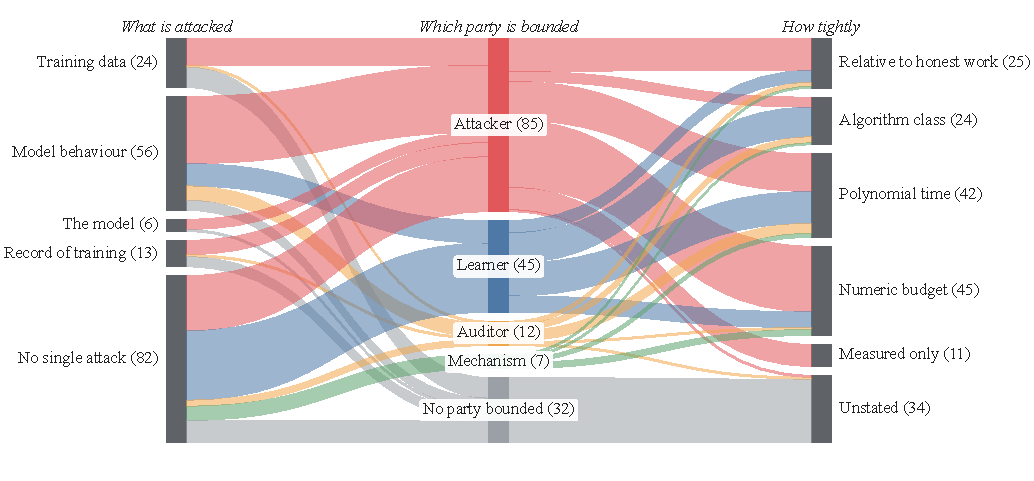
\includegraphics{figures/sankey-corpus}
\caption{The corpus of \NumSources{} works, flowing through what each work
attacks, which party it bounds, and how tightly. Band width is the number of
works and colour is the constrained party. The figure shows three of the thirteen
recorded fields. The full classification is in the supplementary material. Works
with no attack family and works generic over several attacks share the leftmost
band, since neither studies one attack.}
\label{fig:sankey}
\end{figure*}

Figure~\ref{fig:sankey} shows the corpus flowing through three of the recorded
fields. The full classification, on all thirteen fields and with every work named
by citation, is in the supplementary material as six tables. This section reads
them. Each finding names what is dense, what is empty, and what the emptiness
means.

\subsection{The field agrees on access and phase}

The classification by pipeline phase against access level is the one that comes
out full. \NumPhaseAccessCells{} of its 32 cells are populated. Of the \NumAttackWorks{}
works that study an attack, \AttackAccessNamed{} name an access level, and they
split evenly between attacking a model at test time and attacking one already
released. The vocabulary of white box, black box, confidence scores and gradients
is shared, and works from different subfields land in the same cells without
argument.

This is worth establishing before the other three tables, because it shows the
field is capable of agreeing on a threat-model dimension. The disagreement the
rest of this section documents is not a general failure to standardize.

\subsection{It does not agree on resources}

The same corpus against the party each work constrains and the unit it uses fills
\NumPartyUnitCells{} of 75 cells, and the occupied cells do not concentrate. Among the
\NumAttackWorks{} works studying an attack, the adversary is bounded in time in 27
of them, by a perturbation radius in \AttackPerturb{}, in queries in 10, in samples
in 9, and by a corruption fraction in \AttackCorrupt{}. \AttackUnbound{} bound no
party at all.

The row for memory is the one to look at. Four works bound an adversary in memory
and only one of them studies an attack, and that one is bounded-storage
cryptography rather than an attack on a learned model. The bounded-storage
literature has spent two decades on adversaries limited in space, and no work in
this corpus carries that restriction to an adversary attacking a model.

\subsection{The comparable form of bound is almost absent from attack papers}

The third column of Figure~\ref{fig:sankey} sorts the same works by how tightly
each states its bound. \NumExponent{} works state their bound as a relation to an honest party's
work, which is the form that lets two results be placed on one scale.
\NumExponentAttack{} of those \NumExponent{} study an attack, and three of the
\NumExponentAttack{} are cryptographic constructions that happen to carry an attack
family rather than analyses of a deployed system.

The attack literature uses other forms. Of the \NumAttackWorks{} attack works,
\AttackBudget{} state a budget, meaning a numeric allowance such as a perturbation
radius or a query count that carries no relation to anything the defender does.
\AttackUnstated{} state no tightness at all. \AttackPoly{} use the binary
polynomial-time quantifier, \AttackMeasured{} report a measurement with no
definitional standing, and \AttackClass{} name a restricted algorithm class.

A budget bounds what an adversary may change. A relation to honest work bounds what
it must spend to succeed against a defender who spends less. Only the second lets a
reader ask whether one defence costs an attacker more than another, and the corpus
contains \NumExponentAttack{} works that ask it.

\subsection{The attack literature is the half that prices nobody}

Splitting the corpus by whether a work studies a named attack gives the figure's
first column. \AttackUnbound{} of the \NumAttackWorks{} attack works bound no party in
any resource. \TheoryUnbound{} of the \NumTheoryWorks{} works with no attack family
do. Stated as rates, the half of this corpus that studies attacks on machine
learning is about twice as likely to state no adversary bound as the half drawn
from cryptography and learning theory.

The direction is worth stating plainly, because it is the opposite of what a reader
might expect. The cryptographic works in this corpus are not the ones being
imprecise about adversaries. They bound a party in \TheoryUnbound{} fewer cases out
of a smaller total, and when they bound one they more often state the bound in a
form another paper can be compared against.

\subsection{Fifteen works hold a quantity their framing does not carry}

The classification records, separately from how tightly a work states its bound,
whether the work treats that bound as its object or leaves it as a side condition.
Across the corpus the two agree \AssessedPredictable{} per cent of the time, which
is what makes the \NearMiss{} works where they disagree worth naming. Each holds a
resource quantity that its own framing does not carry.

\NearMissA{} of them state a bound in definitional form and do not treat it as the
thing being studied. The filtering impossibility is the clearest. Its theorem turns
on the filter running no faster than the model it audits, which is a ratio between
two parties' compute, and the paper states it as a side condition rather than as the
quantity the result is about \cite{BGGKRR25}. The evaluation guidance that rejects
attacker compute as a threat-model parameter nonetheless fixes a perturbation radius
and reasons about gradient-step counts \cite{CAPBRTGMK19}. Two proof-of-learning
follow-ups price a forgery against honest training and leave the ratio
unparameterized \cite{ZFWCSXZ26}.

\NearMissB{} run the other way, treating a cost deliberately while stating it only
as a measurement. Dziedzic et al.\ calibrate a proof-of-work puzzle to how much a
client has already extracted, which is an adversary priced in compute, with no
definition and no theorem attached \cite{DKLP22}.

The remaining \NearMissC{} state no tightness at all while plainly assessing a
resource. Proof-of-learning requires that forging cost at least as much as training
and states that requirement three times without an exponent, an adversary class or
a security parameter \cite{JYCDTCP21}. The position that membership inference
cannot establish training-set membership rests, in its second and independent
argument, on the cost of sampling a null hypothesis that would require training new
large models \cite{ZDKT25}.

These \NearMiss{} works are where the quantity this survey is about already exists
in the literature without a name.

\subsection{Half the attack literature states no baseline}

An advantage is a success rate minus what public knowledge alone achieves, so a
work that defines adversary success without naming that reference reports a number
with nothing to subtract. \BaselineNA{} of the \NumSources{} works define no
adversary success criterion at all, which is the correct answer for a learning
theory result with no adversary in it. Among the \NumAttackWorks{} works that
study an attack, \BaselineCrit{} define what success means, and of those
\BaselineStated{} name a baseline while \BaselineAbsent{} do not.

This column was the least reliable in the classification and was re-checked in full
before being reported. \BaselineChanged{} of the rows re-checked changed value, and
the errors had four shapes worth naming, because each is a plausible mistake. An
information-theoretic optimum was read as a baseline, when it describes the best any
algorithm could do rather than what an adversary without access achieves. A
previously published accuracy number was read as one, when it describes a different
attack. The cost of an alternative algorithm was read as one. And in an
unforgeability game the raw success tolerance was read as a coin flip, when a search
game has no coin-flip structure at all.

Two independent readers checked overlapping rows and agreed on 24 of 27, which is
the only agreement figure this classification has.
